\section*{Problem 3: Schelling's Segregation}
The simulated dynamics of residential area are shown below. The white spaces represent houses occupied by white people; black spaces represent houses occupied by black; and grey spaces represent empty houses. Figure \ref{0move} to \ref{45move} show the distribution of the black and white people after 0 to 45 moves.


\begin{figure}[htbp]
	\begin{center}
		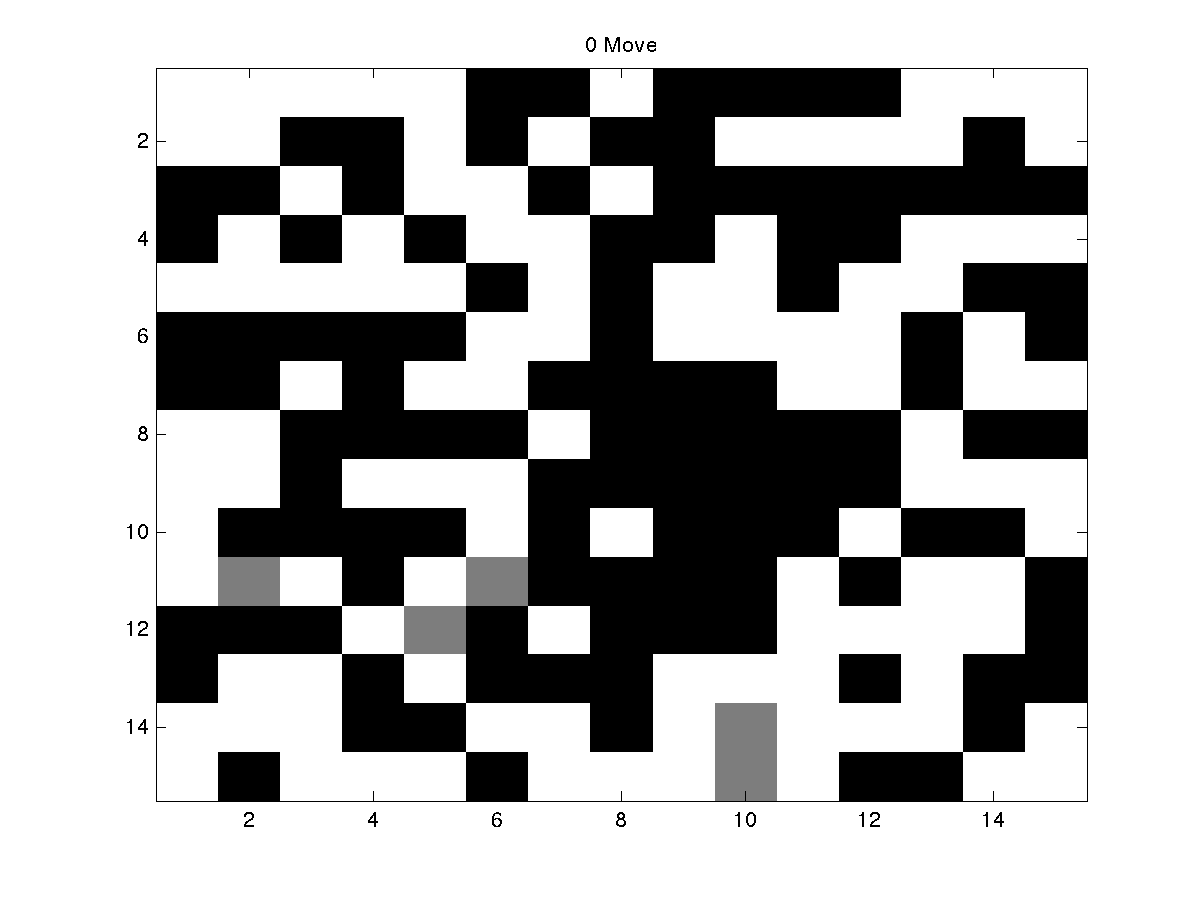
\includegraphics[width=12cm]{Plot/Q3/PS1_Q3_0Move.png}
		\caption{0 Move}
		\label{0move}
	\end{center}
\end{figure}	

\begin{figure}[htbp]
	\begin{center}
		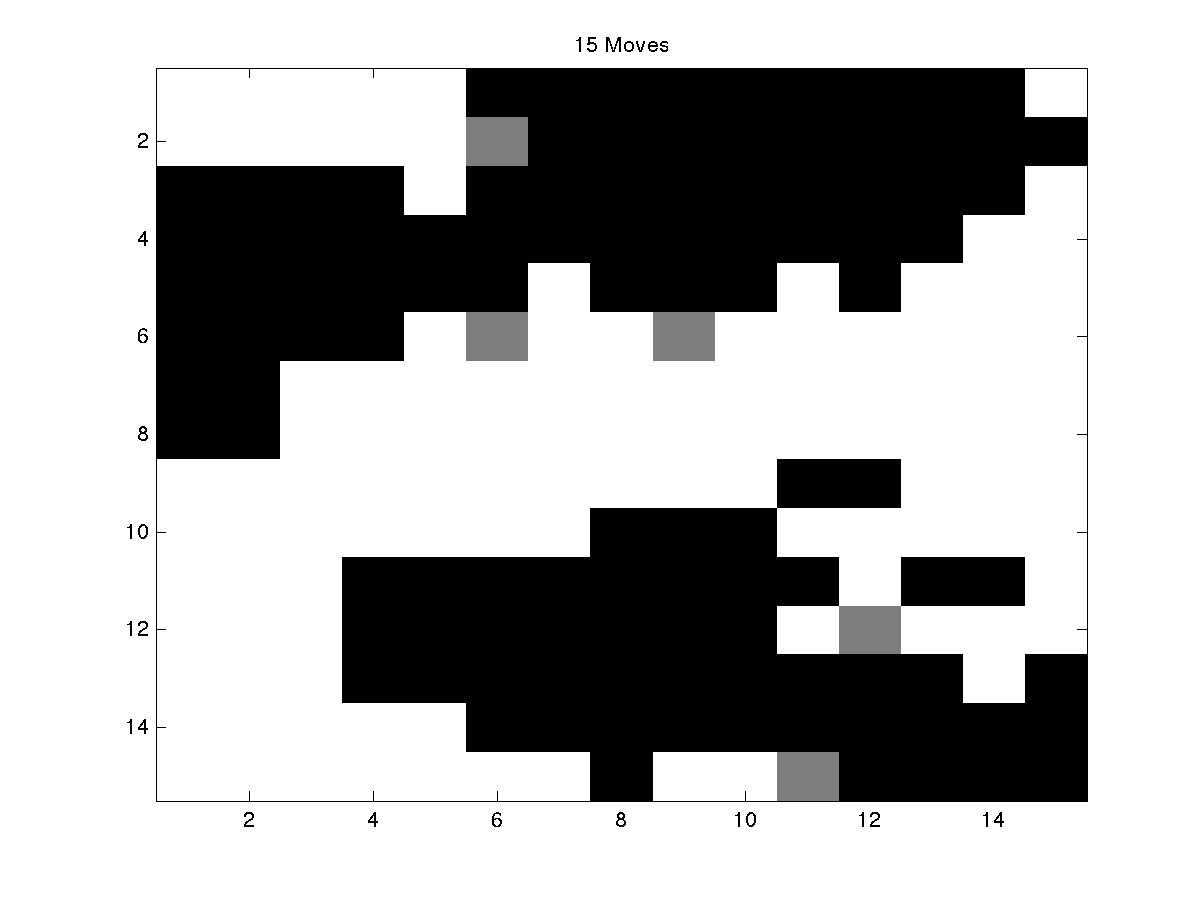
\includegraphics[width=12cm]{Plot/Q3/PS1_Q3_15Move.png}
		\caption{15 Moves}
	\end{center}
\end{figure}

\begin{figure}[htbp]
	\begin{center}
		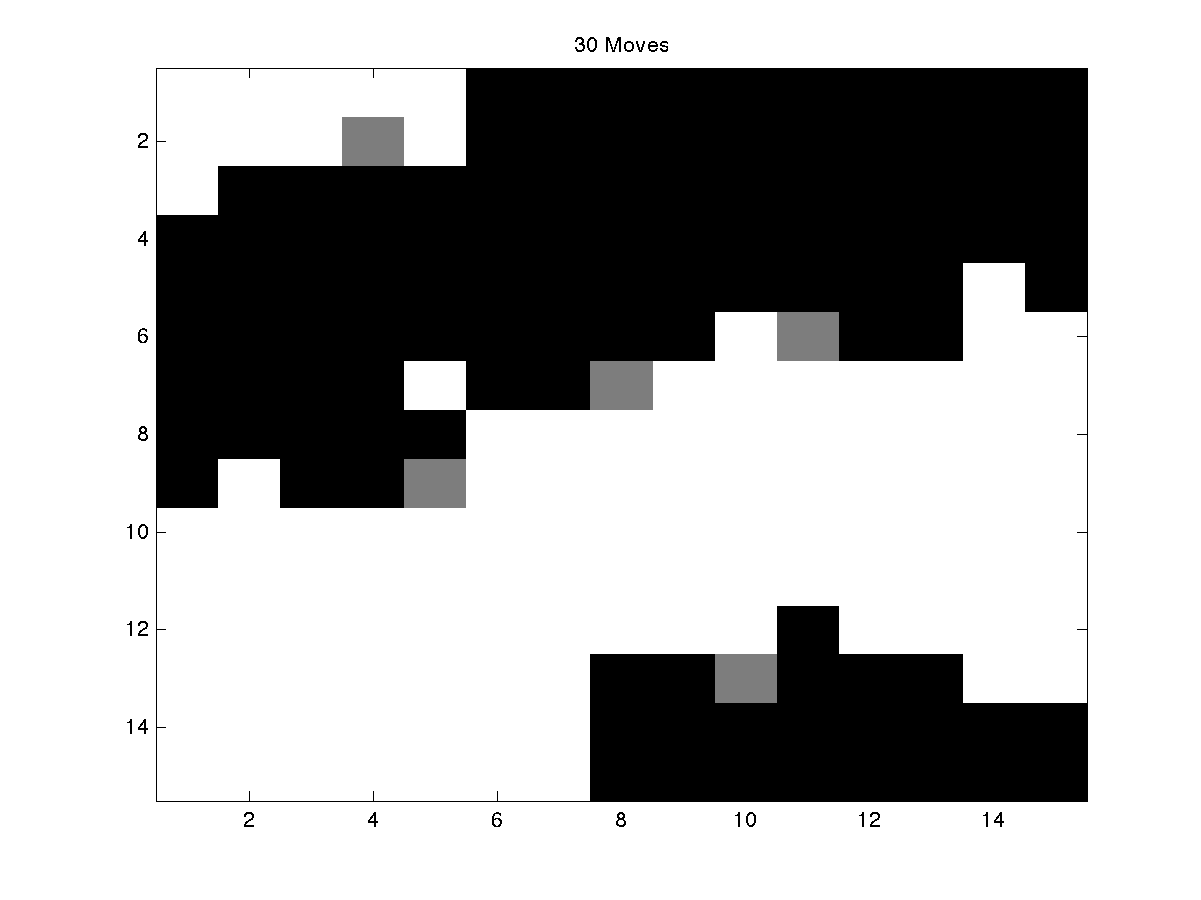
\includegraphics[width=12cm]{Plot/Q3/PS1_Q3_30Move.png}
		\caption{30 Moves}
	\end{center}
\end{figure}	

\begin{figure}[htbp]
	\begin{center}
		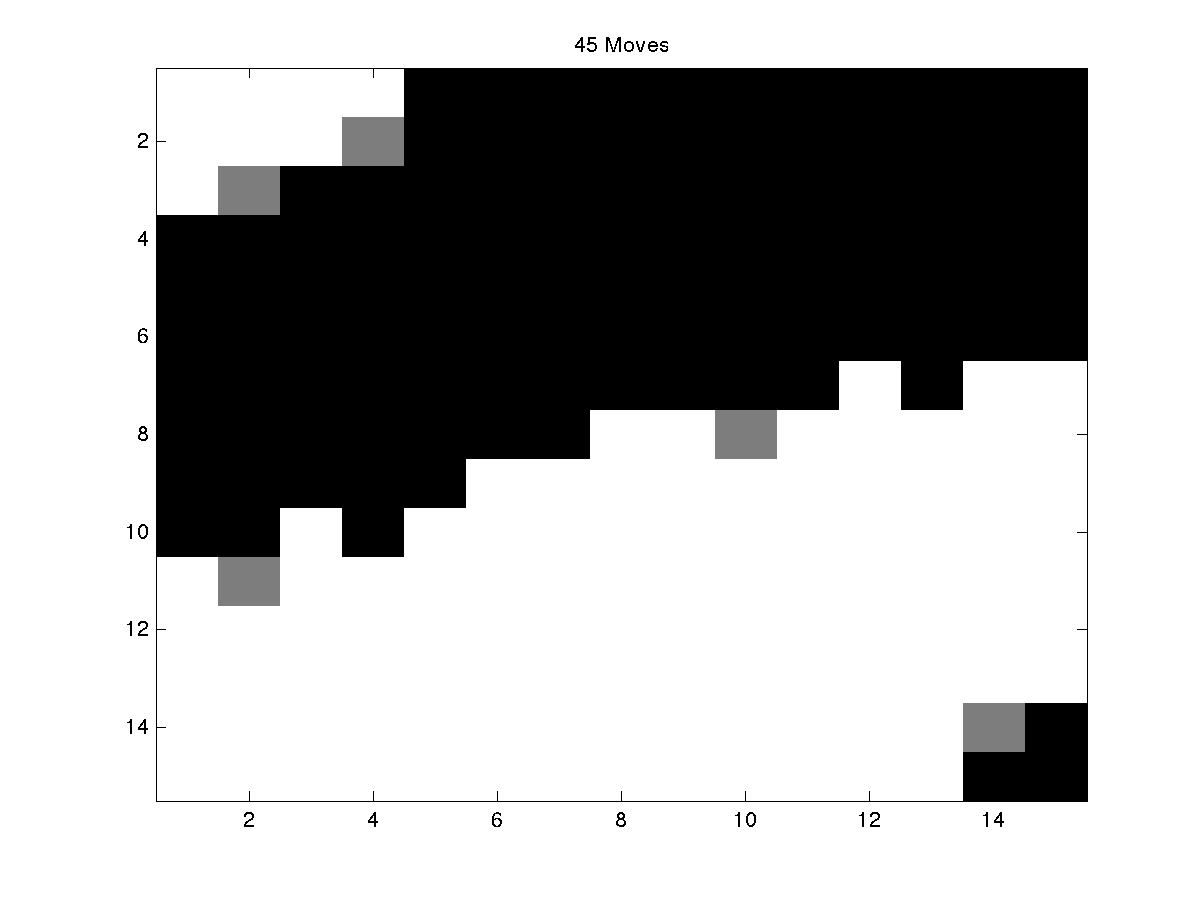
\includegraphics[width=12cm]{Plot/Q3/PS1_Q3_45Move.png}
		\caption{45 Moves}
		\label{45move}
	\end{center}
\end{figure}
